\documentclass{article}

% if you need to pass options to natbib, use, e.g.:
\PassOptionsToPackage{numbers, sort&compress}{natbib}
% before loading neurips_2026

% The authors should use one of these tracks.
% Before accepting by the NeurIPS conference, select one of the options below.
% 0. "default" for submission
\usepackage[main,final]{neurips_2026}
% the "default" option is equal to the "main" option, which is used for the Main Track with double-blind reviewing.
% 1. "main" option is used for the Main Track
%  \usepackage[main]{neurips_2026}
% 2. "position" option is used for the Position Paper Track
%  \usepackage[position]{neurips_2026}
% 3. "eandd" option is used for the Evaluations & Datasets Track
 % \usepackage[eandd]{neurips_2026}
% 4. "creativeai" option is used for the Creative AI Track
%  \usepackage[creativeai]{neurips_2026}
% 5. "sglblindworkshop" option is used for the Workshop with single-blind reviewing
 % \usepackage[sglblindworkshop]{neurips_2026}
% 6. "dblblindworkshop" option is used for the Workshop with double-blind reviewing
 % \usepackage[dblblindworkshop]{neurips_2026}
% 7. "education" option is used for the Education Track
 % \usepackage[education]{neurips_2026}


% After being accepted, the authors should add "final" behind the track to compile a camera-ready version.
% 1. Main Track
 % \usepackage[main, final]{neurips_2026}
% 2. Position Paper Track
% \usepackage[position, final]{neurips_2026}
% 3. Evaluations & Datasets Track
 % \usepackage[eandd, final]{neurips_2026}
% 4. Creative AI Track
% \usepackage[creativeai, final]{neurips_2026}
% 5. Workshop with single-blind reviewing
% \usepackage[sglblindworkshop, final]{neurips_2026}
% 6. Workshop with double-blind reviewing
% \usepackage[dblblindworkshop, final]{neurips_2026}
% Note. For the workshop paper template, both \title{} and \workshoptitle{} are required, with the former indicating the paper title shown in the title and the latter indicating the workshop title displayed in the footnote.
% For workshops (5., 6.), the authors should add the name of the workshop, "\workshoptitle" command is used to set the workshop title.
% \workshoptitle{WORKSHOP TITLE}
% 7. Education Track
% \usepackage[education, final]{neurips_2026}

% "preprint" option is used for arXiv or other preprint submissions
 % \usepackage[preprint]{neurips_2026}

% to avoid loading the natbib package, add option nonatbib:
%    \usepackage[nonatbib]{neurips_2026}

\usepackage[utf8]{inputenc} % allow utf-8 input
\usepackage[T1]{fontenc}    % use 8-bit T1 fonts
\usepackage{hyperref}       % hyperlinks
\usepackage{placeins}
\usepackage{float}
\usepackage{graphicx}       % figures
\usepackage{url}            % simple URL typesetting
\usepackage{booktabs}       % professional-quality tables
\usepackage{amsfonts}       % blackboard math symbols
\usepackage{amsmath}        % math environments
\usepackage{amssymb}        % math symbols
\usepackage{nicefrac}       % compact symbols for 1/2, etc.
\usepackage{microtype}      % microtypography
\usepackage{xcolor}         % colors
\usepackage{textcomp}       % cent sign in the reward table

% Section numbers carry a trailing dot in the heading (cross-references unchanged).
\makeatletter
\renewcommand{\@seccntformat}[1]{\csname the#1\endcsname.\quad}
\makeatother

% Note. For the workshop paper template, both \title{} and \workshoptitle{} are required, with the former indicating the paper title shown in the title and the latter indicating the workshop title displayed in the footnote.
\title{One Shared PPO Policy for Heterogeneous Commercial Building HVAC Control}


% The \author macro works with any number of authors. There are two commands
% used to separate the names and addresses of multiple authors: \And and \AND.
%
% Using \And between authors leaves it to LaTeX to determine where to break the
% lines. Using \AND forces a line break at that point. So, if LaTeX puts 3 of 4
% authors names on the first line, and the last on the second line, try using
% \AND instead of \And before the third author name.


\author{%
  Siddharth S \\
  Independent Researcher \\
  \texttt{sid250581@gmail.com} \\
  % examples of more authors
  % \And
  % Coauthor \\
  % Affiliation \\
  % Address \\
  % \texttt{email} \\
  % \AND
  % Coauthor \\
  % Affiliation \\
  % Address \\
  % \texttt{email} \\
  % \And
  % Coauthor \\
  % Affiliation \\
  % Address \\
  % \texttt{email} \\
  % \And
  % Coauthor \\
  % Affiliation \\
  % Address \\
  % \texttt{email} \\
}


\raggedbottom

\begin{document}
\nocite{goldfeder2024smart,goldfeder2026smart}


\maketitle


\begin{abstract}
Heating, ventilation, and air-conditioning (HVAC) systems govern indoor environmental quality in modern buildings, operating under the dual imperative of minimizing energy consumption while strictly preserving occupant thermal comfort. However, simultaneously satisfying these objectives remains challenging due to complex building thermal dynamics, fluctuating weather, and stochastic occupancy patterns, which differ from one building to the next. In this work, we show that a single shared Proximal Policy Optimization (PPO) policy, trained solely on the joint 3C (comfort, cost, and carbon) reward, achieves robust zero-shot generalization across disparate building environments. Specifically, trained across 30 scenarios spanning six distinct building layouts and five climate zones, the policy scores 0.0165 against 0.0461 for the benchmark's PID controller on 90 held-out months, and holds in a completely unseen Minneapolis climate. Furthermore, our findings remain validated entirely within the benchmark's simulator, leaving sim-to-real transfer to future physical testbed deployments. More broadly, the result suggests that a heterogeneous stock is as much a problem of representation as of control: one fixed layout let a single policy cover buildings from 30 to 85 zones without per-building training.
\end{abstract}


\section{Introduction}

\textbf{Context}: Achieving global decarbonization depends heavily on reducing the environmental footprint of the built environment. According to the United Nations Environment Programme \citep{unep2025buildings} and the International Energy Agency \citep{iea2018futureofcooling}, the buildings and construction sector accounts for 34\% of global energy and process $\text{CO}_2$ emissions. Rather than declining in line with climate targets, sector-wide operational emissions rose from 9.3 $\text{GtCO}_2$ in 2015 to a record 9.8 $\text{GtCO}_2$ in 2023, representing a 5.4\% increase. Commercial (non-residential) buildings alone contribute 10\% of total global emissions \citep{eia2018cbecs}, which constitutes roughly 29.4\% of all building-sector emissions. The operational footprint of these facilities is driven primarily by heating, ventilation, and air-conditioning (HVAC) systems.

\textbf{Building control:} A building's HVAC infrastructure consists of interconnected thermal zones served by a central network of heating, cooling, and air-distribution equipment. A central plant supplies heated and chilled water to air-handling units (AHUs), which condition and distribute air through duct networks, while variable air volume (VAV) boxes regulate the airflow delivered to individual zones through dampers and local reheat coils. A building controller monitors measurements from the zones and central plant and acts at both levels: it sets the plant and air-handler operating points, such as hot-water loop temperature and supply-air temperature, and it positions the zone dampers and reheat valves. Rather than directly setting individual zone temperatures, these commands influence the thermal environment indirectly through the building's HVAC equipment and physical dynamics.

\textbf{Challenges in Smart Building Control:} Controlling HVAC systems in commercial buildings presents several interconnected challenges. \textbf{First}, buildings exhibit substantial thermal inertia: structural mass, floors, and furnishings absorb and release heat gradually, causing the thermal impact of a setpoint adjustment to become apparent only after a significant delay. \textbf{Second}, occupancy decides where the objective is charged. As occupants arrive and depart, thermal and ventilation demand shifts across zones, and the score bills comfort only in occupied zones while it bills energy and carbon at every step. A controller has to hold the band where people are, let the empty zones drift, and it sees only a building-wide occupant count rather than which zone is occupied. \textbf{Third}, the operating point that is efficient depends on the weather outside. The same building needs different supply-water and supply-air temperatures in a cold month and a warm one, so a controller that covers both has to move its operating point with the weather rather than hold one setting. To investigate these challenges, the \textbf{Smart Buildings Control Suite} \citep{goldfeder2024smart} provides a standardized environment comprising measured building data, building-specific calibrated simulation environments, and a common control interface.

\textbf{Key contribution:} We design a shared control architecture that enables standard Proximal Policy Optimization (PPO; \citep{schulman2017proximal}) to operate across heterogeneous building configurations. Implemented within the high-throughput \textbf{PufferLib} framework, our approach uses a single shared policy to control buildings with varying numbers of thermal zones and air-handling units, rather than relying on independently trained controllers. We achieve this through a common slot-based representation with equipment-existence indicators, allowing the policy to accommodate variable building configurations using shared parameters. To address the delayed dynamics of HVAC systems, we incorporate historical thermal information, projected comfort deficits, and airflow-related features into the policy's observations. We also employ bounded Beta action distributions to produce valid control commands at every step. Across all training scenarios, the policy directly optimizes the benchmark's joint 3C objective, balancing thermal comfort, operational cost, and carbon emissions without facility-specific reward tuning.

\section{Related Works}

\textbf{Benchmark:} Reinforcement learning has been applied to HVAC control from individual thermal zones to whole-building energy management \citep{wei2017deep,yu2021review}, and a notable real deployment reports 9\% and 13\% energy savings across two commercial facilities \citep{luo2022controlling}. Interacting with buildings is costly, and model-predictive control needs a calibrated model of every building \citep{afram2014theory}, so the Smart Buildings Control Suite trains agents in calibrated simulators built from real telemetry \citep{blum2019prototyping,goldfeder2024smart}. The Smart Buildings Challenge then adds procedurally generated buildings and held-out configurations, to ask whether a learned controller transfers across unseen buildings and climates \citep{goldfeder2026smart}.

\textbf{Offline and online reinforcement learning:} HVAC control studies differ in how agents acquire their experience. Offline reinforcement learning learns from previously collected logs, which avoids exploration and cannot test alternatives the logs never contain \citep{blad2022data,levine2020offline}. Simulation-based training provides a safer setting for exploring alternative control strategies, while recent studies have also investigated transferring simulation-trained policies to real buildings through online adaptation \citep{coraci2023online}. In this work, we adopt interactive simulation-based PPO training, allowing the policy to learn from newly generated environment experiences rather than relying exclusively on fixed historical trajectories.

\textbf{Scalability and generalization across buildings:} Transfer learning reuses a controller trained on source buildings: cross-building transfer of pretrained DQN controllers \citep{fang2023cross}, multi-source transfer for multi-zone control \citep{hou2024multi}, heterogeneous transfer across buildings with different energy systems and state representations \citep{coraci2024heterogeneous}. Each adapts a pretrained controller to a target building; we instead train one shared policy across heterogeneous buildings at once, without target-specific fine-tuning.

\section{Methods}

\subsection{Problem formulation and control environment}

We formulate building climate control as a discrete-time \textbf{partially observed Markov decision process (POMDP)}, $(\mathcal{S}, \mathcal{A}, \mathcal{T}, \mathcal{R}, \Omega, \mathcal{O}, \gamma)$ \citep{garcia2013mdp,sutton2018reinforcement}. Table~\ref{tab:interface} gives the observation, the hybrid action space and the reward.

\begin{table}[h]
\centering
\small
\renewcommand{\arraystretch}{1.35}
\begin{tabular}{@{}p{0.21\linewidth}p{0.73\linewidth}@{}}
\toprule
Space / representation & Parameters and ranges \\
\midrule
\textbf{Observation ($o_t$)} & Flat float32 vector of building-dependent length ($d$): zone temperatures, heating/cooling setpoints, flows, damper and reheat echoes, AHU supply/static states, loop temperatures and pressures; 16 of the 48 supplied diurnal and weekly harmonics; two comfort flags; building-wide occupancy, $(n-125)/126$. \\
\addlinespace[3pt]
\textbf{Action ($a_t$)} & $a^{\text{cont}}\in[-1,1]^{3K+2V+2}$, $a^{\text{disc}}\in\{0,1\}^{K+1}$. Supply air 285--305 K; supply water 310--350 K; static pressure 0--2000 Pa; loop differential pressure 0--20; damper, reheat and recirculation $[0,1]$; on/off for the $K$ handlers and the pump. \\
\addlinespace[3pt]
\textbf{Reward ($r_t$)} & Comfort $C_1$ (occupancy-weighted productivity, \$300 per occupant-hour), energy cost $C_2$ (hourly electricity price of 16--20\,\textcent/kWh plus a monthly gas price) and carbon emission $C_3$ (hourly grid intensity of 87.8--104.7\,g/kWh plus a constant gas rate); all non-positive, unclipped, and zero at the ideal. \\
\addlinespace[3pt]
\textbf{Horizon} & $\Delta t=300$ s; $T=8{,}640$ steps (30 days); discounted training return with $(\gamma,\lambda)=(0.99,0.95)$; evaluation is the negated undiscounted mean per-step reward, averaged across scenarios. \\
\bottomrule
\end{tabular}
\vspace{4pt}
\caption{The control interface of the benchmark environment.}
\label{tab:interface}
\end{table}

The dynamics are \textbf{deterministic} given the commands and the scenario's weather trace: thermal mass delays the response by minutes to hours. Randomness enters only through occupancy. The controller never sees the full state: the mass temperature inside each control volume, the occupancy of an individual zone (only a building-wide count is reported), and the building's identity, weather name or month (only diurnal and weekly harmonics are given). The policy recovers the missing per-zone and temporal context from history (\S3.3); Appendix~A gives the model and Appendix~B the input contract.

The policy acts \textbf{directly on the equipment}, without a rule-based sequence or safety filters. Whatever behaviour it shows is learned from interaction with the simulator.

{\samepage
Each step returns the benchmark's \textbf{3C reward} in the benchmark's notation,
\[
r_t = 0.6\,C_1 + 0.2\,C_2 + 0.2\,C_3,
\]
where $C_1 \le 0$ is the occupancy-weighted comfort term, scored against the standard thermal-comfort band of the benchmark \citep{ashrae55} (zero inside the band and whenever the building is empty, falling linearly over the first 5 K outside it and quadratically beyond), $C_2 \le 0$ the energy cost and $C_3 \le 0$ the carbon emission. No term is clipped, and the objective is unmodified: no shaping, potential or extra comfort term.
}

% NOTE (content.md, not paper prose): What to move to the appendix so this stays a subsection: the arity formula in words, field ordering and the `_1` collision convention, missing-value fill, the full state enumeration, the exact normalisation denominators, the per-op float32 decode identity, and the two-level score definition with its equation. None of them are needed to follow \S3.2--\S3.5, and all are needed by someone re-implementing you.
% NOTE (content.md, not paper prose): One judgement call worth making deliberately: keep the ``no building identifier'' clause in \S3.1 rather than in \S3.5. It reads there as a property of the interface, not as a defence of a claim, and it is the sentence that makes your generalization result about the policy instead of about the data.

\subsection{GPU-Accelerated Simulation Infrastructure}

To enable large-scale parallel training, we port the complete building simulation environment to CUDA, integrating the environment with PufferLib's vector interface \citep{suarez2024pufferlib} and CUDA graph execution. The port is validated against the reference Python implementation. With double-precision physics, the implementation sustains 12K environment steps per second (SPS) on an NVIDIA L40S and 6.2K SPS on an RTX 3090, while the reference Python simulator reaches about 145 SPS on 12 CPU cores. Implementation details, validation and throughput are in Appendix~A.

\subsection{Shared Policy Architecture and Observation Design}

One policy must control buildings of different size with a single set of weights. We achieve that with two choices: an interface identical for every building, and readouts shared by equipment role rather than by zone.

Buildings differ in their numbers of zones and air handlers, so their raw observations are structurally incompatible. We map every building into the same 983-value vector: 90 zone slots, 9 air-handler slots, one hot-water slot and one global slot. Absent slots are zero, device fields are returned to physical units with the constants the gateway supplies, and each group is put on a fixed scale, so the same slot means the same thing in every building (Figure~\ref{fig:arch}; Appendix~B).
% NOTE: panel (b) of the figure is the padded 90-slot layout (the 54-zone building, 36 of 90
% slots zero). Whether that padding detail is main-text or appendix is still open, so the prose
% pointer to panel (b) is removed for now; restore it if the padding case stays in the main text.

\begin{figure}[h]
\centering
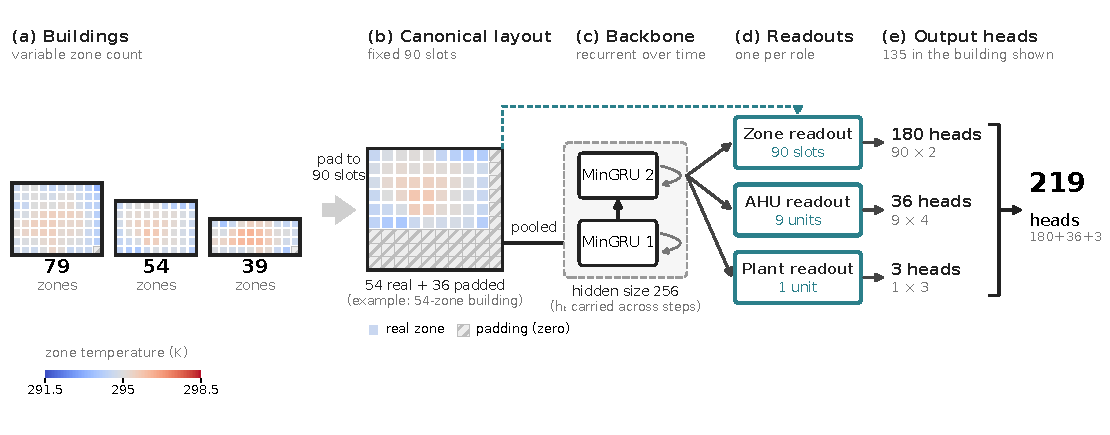
\includegraphics[width=\linewidth]{figures/fig_architecture_v2.pdf}
\caption{Architecture of the shared control policy. (a) Training buildings (79, 54, and 39 zones), zones shaded illustratively by temperature on a shared scale. (b) State slotization: buildings map into 90 fixed zone slots (e.g., 54 active zones and 36 zero-padded slots), 9 AHU slots, 1 plant slot and 1 global slot, 983 values in all. (c) An 80-value pooled summary enters a two-layer recurrent backbone (256 hidden units per layer) that carries one state across steps; each readout also reads its own local slice, 68 values for a zone, 32 for an air handler and 16 for the plant. (d) Shared readout networks grouped by equipment role rather than individual identity. (e) Multi-head policy: 219 heads, 180 for zones (damper and reheat), 36 for AHUs (supply temperature, static pressure, recirculation, on/off) and 3 for the central plant; the pictured building uses 135, and a head a building does not have is masked.}
\label{fig:arch}
\end{figure}

An 80-value pooled summary of that vector (zone and air-handler statistics, plant state, equipment presence, time and occupancy) enters two minimal-GRU layers of 256 hidden units \citep{feng2024rnn}, so the building carries one recurrent state across steps that every slot reads. Each slot's readout combines that state with role-specific local features. For a zone these are its own seven values (temperature, the two setpoint deficits, the heating setpoint, the damper and reheat echoes and presence), the rectified part of each deficit, the eight sensor and echo values of its air handler, and the four sibling entries of every slot in its group, its own included, so a zone is conditioned on its neighbours without a learned attention layer; with the eleven delay features below, a zone reads 68 values, an air handler 32 and the plant 16. Air-handler slots read their own eight values and statistics aggregated over their zones, plus the plant's two loop values. Zone slots also carry a four-hour ring (48 steps) of their own temperature and comfort deficit, from which the history features of Appendix~C are computed.

One readout is shared by every slot of the same role (zone, air handler, plant) rather than learned per zone \citep{zaheer2017deepsets}, so the whole network is 453K parameters shared by all 30 training scenarios. Each zone readout adds a shared 32-unit tanh branch with a zero-initialised output, so at initialisation every head is a fixed affine function of the state and only the nonlinear correction has to be learned. The slot layout has 219 heads; a building masks the ones it does not have and commands between 75 and 209 of them. The critic reads the same trunk state and no input the actor does not see, and it is a state baseline rather than an action-dependent one \citep{tucker2018mirage}. One parameter set therefore serves every zone, air handler and plant in every building.

\subsection{Bounded Action Parameterisation and Policy Optimisation}

\subsubsection{Admissible Control via Bounded Beta Distributions}

To control continuous physical actuators without post-hoc clipping or boundary artefacts, each active head outputs a bounded Beta distribution rather than a standard Gaussian. The policy runs on a padded interface of 256 continuous and 16 discrete heads. It uses 219 continuous heads and no discrete head; a building masks every head it does not have. Rather than squashing an unbounded Gaussian with a $\tanh$ function, which saturates gradients near the limits, or applying an external projection, each head models a Beta distribution over $(0,1)$ \citep{chou2017beta} and emits
\[
a = 2x - 1, \qquad x \sim \operatorname{Beta}(\alpha, \beta);
\]
$a$ is mapped affinely to the range of a continuous command, and the ten on/off commands are read as on when $a > -0.5$.
We compute the shape parameters from the network outputs $u$ and $v$ as
\[
\alpha = \operatorname{softplus}(u) + 0.5, \qquad \beta = \operatorname{softplus}(v) + 0.5.
\]
The $0.5$ floor lets the density form a central mode ($\alpha,\beta>1$) or a bimodal U-shape ($\alpha,\beta<1$), so a damper can be held firmly open or shut; Appendix~H measures which shape the reported policy uses for each actuator. To prevent entropy from vanishing during training, we cap the sum $\alpha+\beta$ at 12: whenever it would exceed 12, both parameters are rescaled by $12/(\alpha+\beta)$, which preserves the mean $\alpha/(\alpha+\beta)$ while bounding policy certainty. Because every sample is natively bounded, all emitted actions are admissible by construction: no external filtering, clipping or projection sits between the policy and the plant (Appendix~D).

\subsubsection{Multi-Head PPO and Horizon Scaling}

Optimising up to 209 actuators at once creates a failure mode for standard policy-gradient updates: a joint ratio lets large steps on a few heads hide behind near-zero shifts on the others. We remove this cross-head interference by decoupling the PPO clipping objective across individual control slots \citep{han2019dimension}. Each active head $h$ keeps its own importance ratio at the stored sample,
\[
r_h(\theta) = \frac{\pi_\theta(x_h \mid s)}{\pi_{\theta_{\mathrm{old}}}(x_h \mid s)}.
\]
Each ratio is clipped independently to $[0.8, 1.2]$, that is $\epsilon = 0.2$, and the surrogate sums these clipped objectives over the building's active heads, $\mathcal{H}$,
\[
\mathcal{L}^{\mathrm{CLIP}}(\theta) = \hat{\mathbb{E}}_t\left[\,\sum_{h\in\mathcal{H}} \min\left(r_{h,t}(\theta)\hat{A}_t,\ \operatorname{clip}\left(r_{h,t}(\theta),\, 1-\epsilon,\, 1+\epsilon\right)\hat{A}_t\right)\right].
\]
The clip keeps each head inside its trust region.

To stabilise learning across buildings with widely differing baseline returns, advantages are standardised over the entire rollout buffer. We set $\gamma = 0.99$ and $\lambda = 0.95$: the return discounts over $1/(1-\gamma) = 100$ steps, eight hours, while the advantage weights a reward $k$ steps back by $(\gamma\lambda)^k$, an effective credit-assignment horizon of about 17 steps \citep{schulman2016gae}, 1.4 hours. That horizon covers the hourly tariff step and the first part of the thermal response, so a price spike attributes credit to the decision that caused it. The policy updates with Adam under a global gradient-norm cap of 0.5, a value coefficient of 0.5, an entropy bonus of 0.001 and a single shared learning rate. We use no reward shaping, potential function or auxiliary objective: the optimisation gradient is the competition score.

\subsubsection{Occupancy-Weighted Zone Critics}

A building-level scalar reward cannot identify which room caused an environmental violation or wasted conditioned air. To direct credit to local actuators without training hundreds of separate networks, we decompose the global reward into per-zone streams,
\[
r_{z,t} = 0.6\,p_{z,t} - 0.2\,s_{z,t}E_t - 0.2\,s_{z,t}C_t, \qquad s_{z,t} = \frac{o_{z,t}}{\sum_{z'} o_{z',t}},
\]
where $p_{z,t}$ measures zone $z$'s local thermal productivity regret, and $E_t$ and $C_t$ are the building's total energy and carbon expenditures. Fuel and carbon costs are allocated to each zone by its share of building occupancy $s_{z,t}$. The allocation conserves on occupied steps: summing the zone streams gives the building-level reward, and an empty building reduces every zone stream to zero.

The critic mirrors this decomposition. Built on the pooled latent representation, the value network outputs one building-level evaluation and 90 parallel zone-level evaluations. The 90 zone predictions share a single value loss, averaged over batch steps and the 90 slots, and their advantages are computed by generalised advantage estimation (GAE). Each zone action head is therefore guided by a local, spatially accurate advantage, giving fine-grained credit across dozens of thermal zones while the network stays single and compact.

\subsection{Training configuration}

\textbf{Scenarios and parallel environments.} Training spans 30 scenarios: six building topologies crossed with five diverse climates (Atlanta, Denver, Fairbanks, Phoenix and Singapore). We run 32 parallel environments per scenario (960 total), collecting 288 steps per worker to yield 276,480 transitions per policy update. Episode starts are staggered per environment, and the scenarios carry different months.

\textbf{Objective, budget and precision.} Training optimises the raw 3C reward of Section 3.1 without modification. The reported policy starts from a fresh random initialisation (seed 75) and runs for 199,895,040 environment steps, 723 rollouts, with the learning rate annealed linearly from $10^{-4}$ to zero over that same budget, so the reported checkpoint is taken at zero step size rather than mid-drift. Adam \citep{kingma2015adam} updates minibatches of 2,304 with four epochs per rollout, the batch design of \citet{andrychowicz2020matters}. The reported run trains on the double-precision solve, as does every score in this paper. A single-precision solve exists as an opt-in speed experiment and is not used here: it moves the observation by about $1.2\times10^{-4}$ against the double-precision reference, ten orders of magnitude above the default path's $2\times10^{-14}$, which is enough to change the reward the policy is trained on (Appendix~A.4). One 46 GB NVIDIA L40S sustains about 12K environment steps per second, so the full run takes roughly 4.6 hours (Appendix~A.3 and Appendix~E).

\section{Results}

Four policies appear in every comparison. \textbf{PID} is the water-based controller the benchmark ships. \textbf{Long} is the earlier 30-scenario run: a 1.5B-step budget with no linear anneal, stopped at 507.6M steps, whose best save is at 89.6M. \textbf{Mid} and \textbf{Final} are two saves of the later 30-scenario run, which budgets 199.9M steps and anneals the learning rate linearly to zero over that budget with a simplified recipe. Mid is the 159.3M save; Final is the 199.1M save, the last complete one and the policy this paper reports. Appendix~E gives both recipes and the checkpoint selection; Appendix~F the metric, the baseline and the public split; Appendix~G the two sets, the 54-month extension and the fuel.

Two held-out sets are reported and never pooled. The first is 90 months: five buildings under 18 weather windows, with two buildings and the Minneapolis climate never trained. The second is a 54-month extension on the three shipped buildings missing from the first set, on the same 18 windows.

\subsection{The score, the terms and the two budgets}

\begin{table}[h!]
\centering
\small
\setlength{\tabcolsep}{4.0pt}
\begin{tabular}{@{}lrrrrrrr@{}}
\toprule
 & steps (M) & comfort & energy & carbon & 90 months & 54 months & public \\
\midrule
\texttt{PID} & -- & 0.0326 & 0.0078 & 0.0057 & 0.0461 & 0.0437 & 0.0640 \\
Long & 507.6 of 1500.2 & 0.0137 & 0.0059 & 0.0057 & 0.0253 & 0.0192 & 0.0182 \\
Mid & 199.9, annealed & 0.0080 & 0.0054 & 0.0051 & 0.0185 & 0.0112 & 0.0175 \\
Final & 199.9, annealed & \textbf{0.0070} & \textbf{0.0051} & \textbf{0.0044} & \textbf{0.0165} & \textbf{0.0098} & 0.0294 \\
\bottomrule
\end{tabular}
\vspace{4pt}
\caption{The four policies on the 90-month set, the 54-month extension and the public leaderboard. The three terms are those of the reward in Section~3.1 with its sign removed, so they sum to the 90-month score; zero is the ideal and lower is better.}
\label{tab:score}
\end{table}


Final scores 0.0165 on the 90 months, 64\% below PID's 0.0461, 35\% below Long's best save and 11\% below Mid, and it is lower than PID on 89 of the 90 months; the exception is \texttt{train\_3}/\texttt{fairbanks\_6}, 0.0459 against 0.0410. On the 54-month extension it is 0.0098, 78\% below PID, 49\% below Long and 13\% below Mid, lower on all 54. Mid takes the public leaderboard, 0.0175 against Final's 0.0294, Long's 0.0182 and PID's 0.0640: the public split (Appendix~F) prefers the mid-anneal save, while the 90 and 54 months and all five buildings prefer Final.


The score is the sum of three terms, and Final's gain is mostly comfort: 0.0070 against 0.0326 for PID, 0.0137 for Long and 0.0080 for Mid, while energy falls from 0.0078 to 0.0051 and carbon from 0.0057 to 0.0044. Comfort is the largest term and the largest fall in every comparison, so no term is bought with another (Table~\ref{tab:score}, Figure~\ref{fig:scores}a).

\begin{figure}[t]
\centering
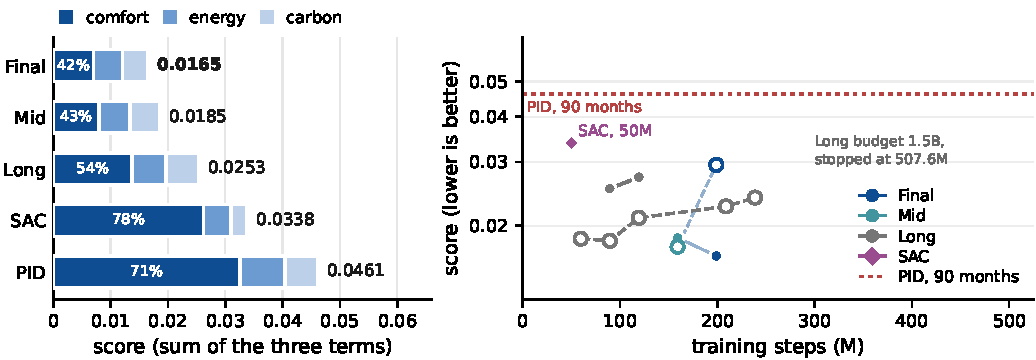
\includegraphics[width=\linewidth]{figures/fig_results_scores_v2.pdf}
\caption{The four policies. (a) The 90-month score as the sum of its three terms, printed at the bar end; comfort is the largest term in every bar. (b) Score against training steps on the 90 months (filled, solid) and on the public leaderboard (open, dashed). Long is best at 89.6M on both and its public score rises afterwards; the later run improves to 199.1M on the 90 months, while its public score is best at 159.3M. The dotted line is \texttt{PID} on the 90 months, comparable only to the filled series.}
\label{fig:scores}
\end{figure}

\FloatBarrier

\subsection{By building and by climate}

Final is below each of the other three on every building and every climate. Its building scores run from 0.0078 on \texttt{train\_2} to 0.0443 on \texttt{train\_3}, below Mid's 0.0087--0.0486, Long's 0.0132--0.0497 and PID's 0.0354--0.0689; its climate scores from 0.0112 in Phoenix to 0.0184 in Fairbanks, below the other three on all six. The two buildings never trained behave like the rest: on \texttt{train\_6} Final is 0.0126 against PID's 0.0491, and on \texttt{train\_3} 0.0443 against 0.0689; the 40 months of the unseen Minneapolis climate are 0.0180 against 0.0519.

\begin{figure}[h]
\centering
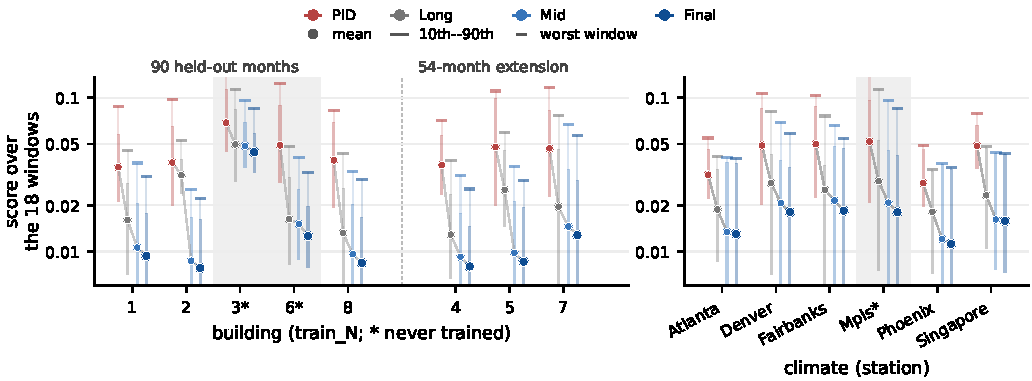
\includegraphics[width=\linewidth]{figures/fig_results_breakdown4_v2.pdf}
\caption{Every building and every climate, four policies. The dot is the mean over the 18 held-out windows of that building or station, the line the 10th to 90th percentile, and the tick the worst window; lower is better. The left block is the 90-month set, the right block the 54-month extension. A star marks a building or station never trained. The order of the four policies is the same inside every range.}
\label{fig:breakdown}
\end{figure}

Figure~\ref{fig:breakdown} shows the distribution behind each mean. Final's worst window is 0.0855 against 0.0960 for Mid, 0.1131 for Long and 0.1625 for PID. \texttt{train\_3} owns all five of its worst months and a fifth of the total (Appendix~F); its 47\% in-band share against 84--98\% elsewhere (Appendix~H) is the residual, not a policy-wide comfort failure. Building identity explains 74\% of the spread in the score and the weather window 22\% (Appendix~G).

On the 54-month extension the buildings are three it trained on, and the windows are the same 18 unseen months. Final is 0.0098, below Mid (0.0112), Long (0.0192) and PID (0.0437) on all 54. The gain is comfort first: occupied zone-steps sit in band 84--98\% of the time on four buildings, \texttt{train\_3} is at 47\%, and the drop against Long is 76\% comfort, 9\% energy and 15\% carbon, while comfort is still 42\% of Final's score, energy 31\% and carbon 27\%. Electricity falls on every building, 73.3 to 45.2\,MWh, gas on three of five, 95.6 to 89.1, and CO$_2$ on four of five, 24.6 to 20.6\,t; gas rises in the two largest plants and CO$_2$ in one, so the total is not a fuel swap (Appendix~G).

\subsection{By time of day and by month}

Final is cheapest while the building is occupied: 0.021--0.041 per step between 06:00 and 19:00, against 0.024--0.045 for Mid, 0.038--0.051 for Long and 0.066--0.131 for PID. At 06:00, the hour the building fills, it is 0.041 against 0.045, 0.051 and 0.131. The weekday night is the only bin where Final is worse than PID, by 20\% (0.0045 against 0.0037); Mid and Long are worse there, 0.0064 and 0.0049.

Figure~\ref{fig:time} breaks the same recording three ways. By hour, the four separate in the occupied window and converge at night. By day-part, the weekday morning is the largest bill for every policy, and weekends are 29\% of the steps with 0.2\% of the electricity and 0.7\% of the gas. By month, the cold windows carry the bill and the warm ones are nearly free; Final is lowest in every month, from 0.033 in January to 0.009 in August, and \texttt{train\_3} drifts by $3.8\times10^{-4}$ per day, about 0.011 over the month (Appendix~H).

\begin{figure}[h]
\centering
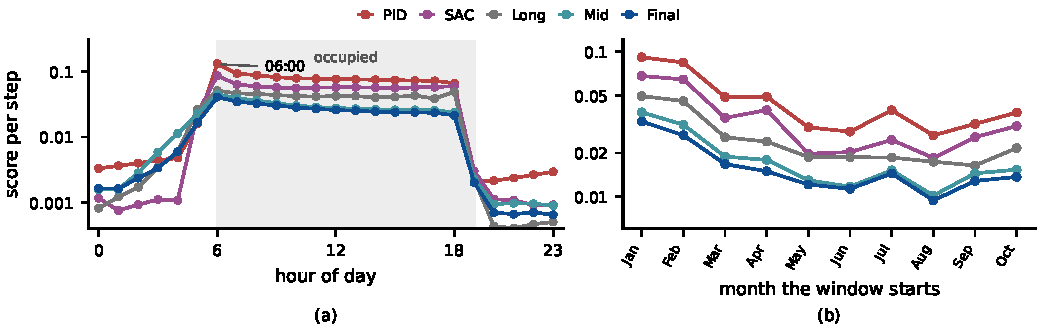
\includegraphics[width=0.9\linewidth]{figures/fig_results_time4.pdf}
\caption{The same recording by hour, by day-part and by month. (a) Score per step by hour of day, on a log scale; the shaded band is the occupied window, and 06:00 is the most expensive hour for every policy. (b) Weekday night, morning, afternoon and evening and the weekend, log scale. (c) The month each window starts, January to October. Lower is better throughout.}
\label{fig:time}
\end{figure}

It does not save by switching equipment off; it saves by choosing when the building is conditioned (Appendix~H).

\section{Conclusion}
\label{sec:conclusion}

A single 453K-parameter policy, trained once across six buildings and five climates, was evaluated across eight buildings and six climates. It achieves scores of 0.0165 on the 90 held-out months and 0.0098 on the 54-month extension, compared to 0.0461 and 0.0437 for the benchmark's default controller. More consequential than the mean score is its variance structure: 74\% of the score spread is attributable to building identity and only 22\% to weather, directly inverting the baseline's sensitivity. The policy decouples control performance from seasonal variation, leaving building-specific dynamics as the primary residual.

Three things bound that claim. It is one seed. Some noise remains in the reported score, and the recipe was not tested with ablations at this scale, one change at a time. And the baseline is the controller the benchmark ships, untuned: no tuned classical controller and no other reinforcement-learning algorithm was run against it.

Three tests follow. First, our reported experiments were conducted on the original, \textbf{unpatched} benchmark release; this comparison must be replicated on the corrected environment alongside official entrant submissions. Second, multi-seed evaluations are required to quantify performance variance. Third, the policy must be benchmarked against stronger reinforcement learning baselines.


\clearpage
\bibliographystyle{unsrtnat}
\nocite{*}
\bibliography{references}

\end{document}
